\chapter{Настройка оптического интерферометра методами машинного обучения с подкреплением}\label{ch:ch2}

\section{Физические принципы работы и модель оптического интерферометра}\label{sec:ch2/sec1}

\subsection{Математическая модель интерференции света}

Работа оптического интерферометра основана на принципе интерференции света --- физического процесса при котором два когерентных световых пучка накладываются друг на друга и образуют в пространстве периодическую структуру состоящую из минимумов и максимумов интенсивности получившую название интерференционной картины. 

\begin{figure}[ht]
    \centerfloat{
        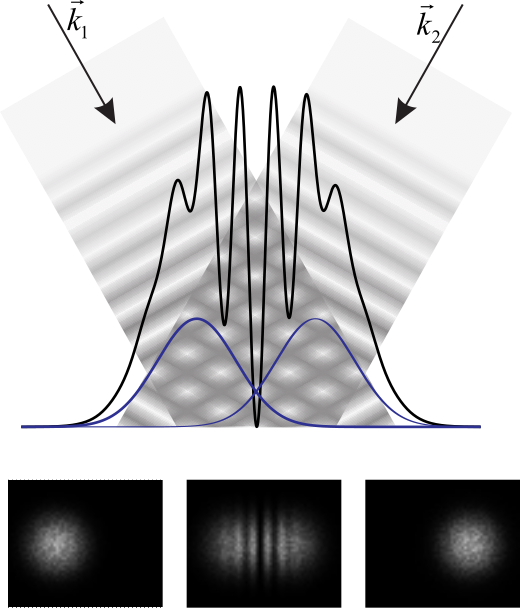
\includegraphics[scale=1.7]{images/interf_expl.png}
    }
    \caption{Одномерный срез интерференционной картины полученный при неполном перекрытии двух когерентных лазерных лучей с волновыми векторами $k_1$ и $k_2$. Волновые фронты показаны с помощью градиента; голубые линии показывают интенсивности индивидуальных лучей (не в масштабе); черные линии соответствуют профилю интенсивности результирующей картины. Соответствующие двумерные изображения индивидуальных лучей и их интерференционной картины представлены внизу.}\label{fig:two_beam_interf}
\end{figure}

Интерференционная картина получаемая при наложении двух когерентных лучей изображена на рис. \ref{fig:two_beam_interf}. Для вычисления интерференционной картины опишем математическую модель интерференции. Рассмотрим световой пучок распространяющийся вдоль оси $z$ в параксиальном приближении $k_z \gg k_x, k_y$, где волновой вектор $\vec{k}$ --- вектор, направление которого перпендикулярно фазовому фронту волны, а абсолютное значение равно волновому числу. Волновое число $k$ связано с длинной волны $\lambda$ соотношением 

\begin{equation*}
    k = \frac{2\pi}{\lambda}
\end{equation*}

Распределение амплитуды излучения будем описывать с помощью нормального распределения. Определим радиус пучка $r$ как расстояние от центра пучка на котором напряженность электромагнитного поля падает в $e$ раз. 
Тогда распределение напряженности электромагнитного поля в каждом световом пучке $E(x, y, z)$ задается следующим выражением: 

\begin{equation}
    E(x,y,z) = e^{-\frac{(x-x_0(z))^2+(y-y_0(z))^2}{r^2}} e^{i k_xx+ik_yy+ik_zz}    
\label{eq:Exyzt}
\end{equation}

где $(x,y,z)$ координатный вектор, $(x_0(z),y_0(z))$ положение центра пучка, $\vec{k}$ волновой вектор $r$ радиус пучка. %We neglect the beam divergence due to diffraction.
Первый множитель уравнения \ref{eq:Exyzt} соответствует амплитуде электромагнитной волны $A(x,y,z)$, а второй --- фазе $\exp(i\phi(x,y,z))$. 
При сложении двух электромагнитных волн в точке $x, y, z$ итоговая напряженность поля будет равна сумме напряженностей отдельных волн: 

\begin{equation}
    E(x, y, z) = E_1(x, y, z) + E_2(x, y, z)
\label{eq:E1E2}
\end{equation}

Видимая интерференционная картина определяется распределением интенсивности света, которая равна квадрату модуля напряженности электромагнитного поля: 

\begin{equation}
    I(x, y, z) = |E(x, y, z)|^2 = E(x,y,z) E^*(x,y,z)
\label{eq:ie2}
\end{equation}

Таким образом в соответствии с уравнениями \ref{eq:Exyzt}, \ref{eq:E1E2}, \ref{eq:ie2} интенсивность света в точке $x, y, z$ сложении двух световых лучей определятся выражением: 

\begin{multline}
    I(x, y, z) = E_1E_1^* + E_2E_2^* + E_1E_2^* + E_2E_1^* = \\
    I_1(x,y,z) + I_2(x,y,z) + 2 \sqrt{I_1(x,y,z)I_2(x,y,z)}\cos(\Delta \phi)
\label{eq:interf}
\end{multline}

где $\Delta \phi = \phi_1 - \phi_2$ --- разность фаз двух волн. Из уравнения \ref{eq:interf} следует, что если две волны складываются синфазно т.е. $\Delta \phi = 0$, то интенсивность света максимальна $I = I_1 + I_2 + 2\sqrt{I_1I_2}$. Если же две волны складываются в противофазе т.е. $\Delta \phi = \pi$, то интенсивность света минимальна $I = I_1 + I_2 - 2\sqrt{I_1I_2}$.

\subsection{Математическая модель интерферометра Маха-Цендера}

Интерферометры являются одними из основных инструментов в экспериментальной оптике и служат для прецизионного измерения разности фаз между двумя лучами. Интерферометр Фабри-Перо\cite{fabry-perot1899} используется в оптической спектрометрии; интерферометр Майкельсона является основной частью современных детекторов гравитационных волн LIGO и VIRGO \cite{LIGO, VIRGO} он также используется для измерения шероховатости поверхностей; интерферометр Саньяка используется в современных навигационных системах; интерферометр Маха-Цендера является основным инструментом в современных экспериментах в квантовой оптике \cite{Sarkar2006, Sychev2017}. 

В рамках данной работы рассматривалась настройка оптического интерферометра Маха-Цендера методами машинного обучения с подкреплением. Схема работы интерферометра Маха-Цендера изображена на рис. \ref{fig:MZI}. 

\begin{figure}[ht]
\centerfloat{
    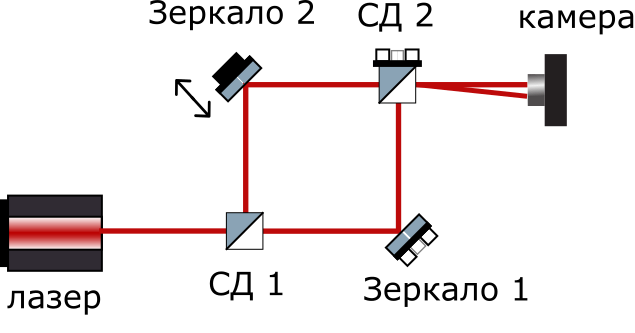
\includegraphics[scale=2.0]{images/MZI_expl.png}
}
\caption{Принципиальная схема работы интерферометра Маха-Цендера}
\label{fig:MZI}
\end{figure}

В ней лазерный луч после прохождения светоделителя СД 1 разделяется на два луча. Верхний луч проходит через зеркало 2 и светоделитель СД 2 и попадает на камеру. Нижний луч проходит через светоделитель СД 1 и зеркало 1. Для настройки интерферометра необходимо точно совместить два луча как по положению, так и по направлению на камере. Регулировка нижнего луча производится с помощью зеркала 1 и светоделителя СД 2. Верхний луч является неподвижным. Настройка интерферометра представляет собой итеративный процесс в котором человек ориентируясь на интерференционную картину, получаемую на камере подстраивает положение зеркала 1 и светоделителя 2, чтобы добиться идеального совпадения лучей. Для визуализации разности фаз между двумя плечами интерферометра зеркало 2 совершает колебательные движения на расстояние порядка длины волны $\lambda$ благодаря чему фаза верхнего луча изменяется в интервале $\phi \in [0, 2\pi)$. Настройка интерферометра представляет собой трудоемкий процесс осложненный тем, что и зеркало 1 и светоделитель СД 2 меняют одновременно и положение луча на камере и угол между лучами. 

\begin{figure}[ht]
\centerfloat{
    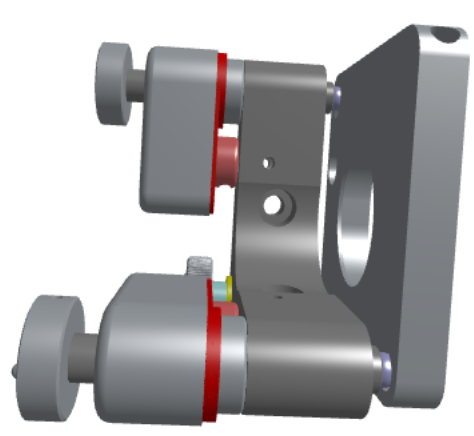
\includegraphics[scale=0.3]{images/mirror_mount.png}
}
\caption{3D модель крепления оптического зеркала использованного в работе \cite{newport_mirror}}
\label{fig:mirror}
\end{figure}

На рис. \ref{fig:mirror} показана 3D модель крепления оптического зеркала использованная в работе для регулировки положения зеркала 1 и светоделителя СД 2. Крепление оборудовано двумя микрометрическими винтами которые также могут управляться с помощью встроенных пьезо двигателей. Каждый из винтов поворачивает зеркало вокруг перпендикулярных плоскостей. Направление вектора нормали зеркала $\vec{n}$ зависит от положений винтов $x, y$ в приближении малых углов следующим образом: 

\begin{equation}
    \vec{n} = \begin{pmatrix}
        x\\ 
        y\\ 
        \sqrt{1 - x^2 - y^2}
    \end{pmatrix}
\end{equation}


Для вычисления интерференционной картины по формуле \ref{eq:interf} необходимо знать положение центров лучей на камере и их фазы. Предполагаем, что верхний луч распространяется точно вдоль оси  $z$, таким образом для него $x_0\equiv y_0\equiv k_x\equiv k_y\equiv 0$. Для нижнего луча в работе производится трассировка нижнего луча через систему зеркал. Введем систему координат с центром в камере как показано на рис. \ref{fig:MZI_coordis}. 


\begin{figure}[ht]
\centerfloat{
    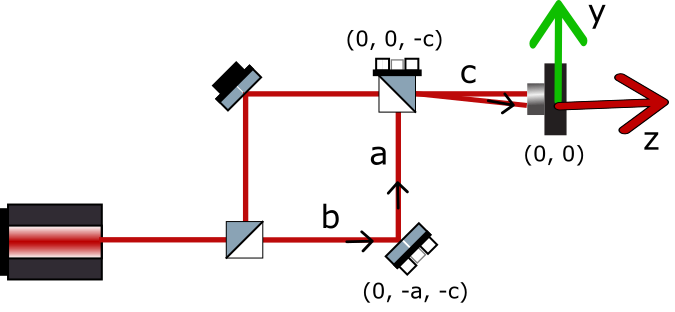
\includegraphics[scale=2.0]{images/MZI_matmodel.png}
}
\caption{Система координат}
\label{fig:MZI_coordis}
\end{figure}

При прохождении каждого зеркала находится точка пересечения луча с плоскостью зеркала и рассчитывается угол поворота луча. Луч вращается относительно плоскости перпендикулярной плоскости образованной вектором нормали зеркала и первоначальным направлением луча. Величина угла определяется из закона отражения. Листинг функции трассировки приведен в приложении \ref{lst:beam_trace}.


\subsection{Видность интерференционной картины}

Интенсивность интерференционной картины получаемой при наложении двух лучей в плоскости камеры ($z=0$) задается выражением:

\begin{equation}
    I(x,y,t)=|E_1(x,y,0)+E_2(x,y,0)e^{i\phi_{\mathrm{piezo}}(t)}|^2  
\end{equation}

где $\phi_{\mathrm{piezo}}(t)$ фазовый сдвиг получаемый из-за движения пьезо зеркала. Таким образом разность фаз $\Delta \phi$ в уравнении \ref{eq:interf} за один проход пьезо зеркала пробегает интервал от $0$ до $2\pi$. Суммарной интенсивностью интерференционной картины называется величина: 

\begin{equation}
    I_{\mathrm{tot}}(t) = \iint_{-\infty}^{+\infty} I(x, y, t) {\mathrm{d}}x{\mathrm{d}}y
\end{equation}

Периодическое движение пьезо зеркала приводит к периодическому изменению суммарной интенсивности. Пример изменения интенсивности интерференционной картины показан на рис. \ref{fig:intens_plot}.

\begin{figure}[ht]
\centerfloat{
    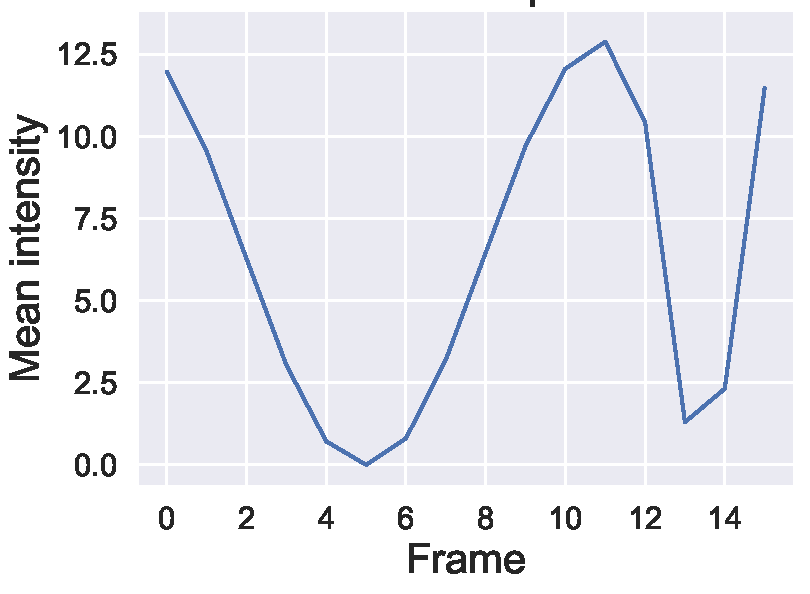
\includegraphics[scale=0.7]{images/piezo_intens_plot.pdf}
}
\caption{График изменения интенсивности (слева) и график движения пьезо зеркала (справа) TODO}
\label{fig:intens_plot}
\end{figure}

Основным критерием качества настройки интерферометра является видность интерференционной картины: 

\begin{equation}
    V = \frac{            
        \max_{t}(I_{\mathrm{tot}}) - \min_t(I_{\mathrm{tot}})}
        {\max_{t}(I_{\mathrm{tot}}) + \min_t(I_{\mathrm{tot}})}
    \label{eq:visib}
\end{equation}

Видность интерференционной картины вычисляется с помощью минимума $\min_t(I_{\mathrm{tot}})$ и максимума $\max_t(I_{\mathrm{tot}})$ суммарной интенсивности света на камере. Максимум и минимум вычисляются за один полный период прохода пьезо зеркала. По определению видность является действительным числом и находится в интервале $V \in [0, 1]$. 

Примеры интерференционных картин и графики соответствующих им суммарных интенсивностей приведены на рис. \ref{fig:visib_expl}. Для полностью настроенного интерферометра [рис.~\ref{fig:visib_expl}(a)], $\min_t(I_{\mathrm{tot}})=0$, таким образом видность $V=1$, для полностью расстроенного интерферометра [Fig.~\ref{fig:visib_expl}(c)], $\min_t(I_{\mathrm{tot}})\approx\max_t(I_{\mathrm{tot}})$, таким образом видность $V\approx 0$.

\begin{figure}[ht]
\centerfloat{
    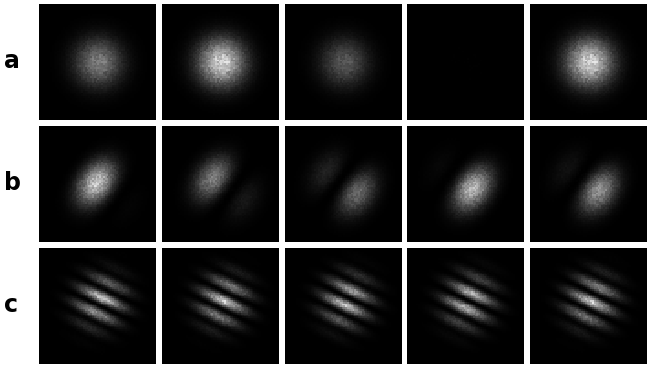
\includegraphics[scale=0.7]{images/visib_expl.png}
}
\caption{Примеры интерференционных картин полученные в симуляции. (a) Полностью настроенный интерферометр, видность = 1; (b) Слабо расстроенный интерферометр, видность = 0.3; (c) Сильно расстроенный интерферометр, видность =
0.0026. Изображения слева на право соответствуют различной разности фаз [$\phi_{\mathrm{piezo}}(t)$] между двумя плечами интерферометра из-за движения пьезо зеркала}
\label{fig:visib_expl}
\end{figure}


Из уравнений.~\eqref{eq:Exyzt} и \eqref{eq:visib}, получим точное выражение для видности интерференционной картины:

\begin{equation}
    V = \exp\left(- \frac{x_0^2 + y_0^2}{2 r^2}\right)  \exp\left[- \frac{(k_x^2 + k_y^2) r^2}{8}\right],
    \label{eq:visib_rot}
\end{equation}

где $x_0$ и $y_0$ координаты центра нижнего луча на камере; $k_x$ и $k_y$ компоненты волнового вектора нижнего луча. Вывод уравнения \ref{eq:visib_rot} приведен в приложении \ref{app:B1}.

\subsection{Математическая модель интерферометра Маха-Цендера с линзами}

Интерферометр Маха-Цендера показанный на рис.


\subsection{Видность интерференционной картины в интерферометре Маха-Цендера с линзами}

\subsection{Численная модель интерферометра Маха-Цендера}

python, C++, threads, camera pixel parallel computation


\section{Настройка оптического интерферометра как задача машинного обучения с подкреплением}\label{sec:ch2/sect2}

А это две картинки под общим номером и названием:
\begin{figure}[ht]
    \begin{minipage}[b][][b]{0.49\linewidth}\centering
        \includegraphics[width=0.5\linewidth]{knuth1} \\ а)
    \end{minipage}
    \hfill
    \begin{minipage}[b][][b]{0.49\linewidth}\centering
        \includegraphics[width=0.5\linewidth]{knuth2} \\ б)
    \end{minipage}
    \caption{Очень длинная подпись к изображению,
        на котором представлены две фотографии Дональда Кнута}
    \label{fig:knuth}
\end{figure}

Те~же~две картинки под~общим номером и~названием,
но с автоматизированной нумерацией подрисунков:
\begin{figure}[ht]
    \centerfloat{
        \hfill
        \subcaptionbox[List-of-Figures entry]{Первый подрисунок\label{fig:knuth_2-1}}{%
            \includegraphics[width=0.25\linewidth]{knuth1}}
        \hfill
        \subcaptionbox{\label{fig:knuth_2-2}}{%
            \includegraphics[width=0.25\linewidth]{knuth2}}
        \hfill
        \subcaptionbox{Третий подрисунок, подпись к которому
            не~помещается на~одной строке}{%
            \includegraphics[width=0.3\linewidth]{example-image-c}}
        \hfill
    }
    \legend{Подрисуночный текст, описывающий обозначения, например. Согласно
        ГОСТ 2.105, пункт 4.3.1, располагается перед наименованием рисунка.}
    \caption[Этот текст попадает в названия рисунков в списке рисунков]{Очень
        длинная подпись к второму изображению, на~котором представлены две
        фотографии Дональда Кнута}\label{fig:knuth_2}
\end{figure}

На рисунке~\cref{fig:knuth_2-1} показан Дональд Кнут без головного убора.
На рисунке~\cref{fig:knuth_2}\subcaptionref*{fig:knuth_2-2}
показан Дональд Кнут в головном уборе.

Возможно вставлять векторные картинки, рассчитываемые \LaTeX\ <<на~лету>>
с~их~предварительной компиляцией. Надписи в таких рисунках будут выполнены
тем же~шрифтом, который указан для документа в целом.
На~рисунке~\cref{fig:tikz_example} на~странице~\pageref{fig:tikz_example}
представлен пример схемы, рассчитываемой пакетом \verb|tikz| <<на~лету>>.
Для ускорения компиляции, подобные рисунки могут быть <<кешированы>>, что
определяется настройками в~\verb|common/setup.tex|.
Причём имя предкомпилированного
файла и~папка расположения таких файлов могут быть отдельно заданы,
что удобно, если не~для подготовки диссертации,
то~для подготовки научных публикаций.
\begin{figure}[ht]
    \centerfloat{
        \ifdefmacro{\tikzsetnextfilename}{\tikzsetnextfilename{tikz_example_compiled}}{}% присваиваемое предкомпилированному pdf имя файла (не обязательно)
        \input{Dissertation/images/tikz_scheme.tikz}

    }
    \legend{}
    \caption[Пример \texttt{tikz} схемы]{Пример рисунка, рассчитываемого
        \texttt{tikz}, который может быть предкомпилирован}\label{fig:tikz_example}
\end{figure}

Множество программ имеют либо встроенную возможность экспортировать векторную
графику кодом \verb|tikz|, либо соответствующий пакет расширения.
Например, в GeoGebra есть встроенный экспорт,
для Inkscape есть пакет svg2tikz,
для Python есть пакет tikzplotlib,
для R есть пакет tikzdevice.

\section{Настройка интерферометра с использованием дискретных действий}\label{sec:ch2/sec3}

\subsection{Дискретизация пространства действий}
\subsection{Функция награды}

\noindent Нумерованный список:
\begin{enumerate}
    \item Первый пункт.
    \item Второй пункт.
    \item Третий пункт.
\end{enumerate}

\noindent Маркированный список:
\begin{itemize}
    \item Первый пункт.
    \item Второй пункт.
    \item Третий пункт.
\end{itemize}

\noindent Вложенные списки:
\begin{itemize}
    \item Имеется маркированный список.
          \begin{enumerate}
              \item В нём лежит нумерованный список,
              \item в котором
                    \begin{itemize}
                        \item лежит ещё один маркированный список.
                    \end{itemize}
          \end{enumerate}
\end{itemize}

\noindent Нумерованные вложенные списки:
\begin{enumerate}
    \item Первый пункт.
    \item Второй пункт.
    \item Вообще, по ГОСТ 2.105 первый уровень нумерации
          (при необходимости ссылки в тексте документа на одно из перечислений)
          идёт буквами русского или латинского алфавитов,
          а второй "--- цифрами со~скобками.
          Здесь отходим от ГОСТ.
          \begin{enumerate}
              \item в нём лежит нумерованный список,
              \item в котором
                    \begin{enumerate}
                        \item ещё один нумерованный список,
                        \item третий уровень нумерации не нормирован ГОСТ 2.105;
                        \item обращаем внимание на строчность букв,
                        \item в этом списке
                              \begin{itemize}
                                  \item лежит ещё один маркированный список.
                              \end{itemize}
                    \end{enumerate}

          \end{enumerate}

    \item Четвёртый пункт.
\end{enumerate}

\section{Настройка интерферометра с использованием непрерывных действий}

Много полезных советов приведено в материале
<<\href{https://kostyrka.ru/main/ru/typesetting-and-typography-crash-course-by-kostyrka/}{Краткий курс благородного набора}>>
(автор А.\:В.~Костырка).
Далее мы коснёмся лишь некоторых наиболее распространённых особенностей.

\subsection{Пространство действий}

В~русском наборе принято:
\begin{itemize}
    \item единицы измерения, знак процента отделять пробелами от~числа:
          10~кВт, 15~\% (согласно ГОСТ 8.417, раздел 8);
    \item \(\tg 20\text{\textdegree}\), но: 20~{\textdegree}C
          (согласно ГОСТ 8.417, раздел 8);
    \item знак номера, параграфа отделять от~числа: №~5, \S~8;
    \item стандартные сокращения: т.\:е., и~т.\:д., и~т.\:п.;
    \item неразрывные пробелы в~предложениях.
\end{itemize}

\subsection{Функция награды}

Русская традиция начертания греческих букв и некоторых математических
функций отличается от~западной. Это исправляется серией
\verb|\renewcommand|.
\begin{itemize}
    %Все \original... команды заранее, ради этого примера, определены в Dissertation\userstyles.tex
    \item[До:] \( \originalepsilon \originalge \originalphi\),
          \(\originalphi \originalleq \originalepsilon\),
          \(\originalkappa \in \originalemptyset\),
          \(\originaltan\),
          \(\originalcot\),
          \(\originalcsc\).
    \item[После:] \( \epsilon \ge \phi\),
          \(\phi \leq \epsilon\),
          \(\kappa \in \emptyset\),
          \(\tan\),
          \(\cot\),
          \(\csc\).
\end{itemize}

Кроме того, принято набирать греческие буквы вертикальными, что
решается подключением пакета \verb|upgreek| (см. закомментированный
блок в~\verb|userpackages.tex|) и~аналогичным переопределением в
преамбуле (см.~закомментированный блок в~\verb|userstyles.tex|). В
этом шаблоне такие переопределения уже включены.

Знаки математических операций принято переносить. Пример переноса
в~формуле~\eqref{eq:equation3}.

В английском языке приняты одинарные и двойные кавычки в~виде ‘...’ и~“...”.
В~России приняты французские («...») и~немецкие („...“) кавычки (они называются
«ёлочки» и~«лапки», соответственно). ,,Лапки`` обычно используются внутри
<<ёлочек>>, например, <<... наш гордый ,,Варяг``...>>.

Французкие левые и правые кавычки набираются
как лигатуры \verb|<<| и~\verb|>>|, а~немецкие левые
и правые кавычки набираются как лигатуры \verb|,,| и~\verb|‘‘| (\verb|``|).

Вместо лигатур или команд с~активным символом "\ можно использовать команды
\verb|\glqq| и \verb|\grqq| для набора немецких кавычек и команды \verb|\flqq|
и~\verb|\frqq| для набора французских кавычек. Они определены в пакете
\verb|babel|.

%  babel+pdflatex по умолчанию, в polyglossia надо включать опцией (и перекомпилировать с удалением временных файлов)
Команда \verb|"---| используется для печати тире в тексте. Оно может быть
несколько короче английского длинного тире (подробности в~документации
русификации babel). Кроме того, команда задаёт небольшую жёсткую отбивку
от~слова, стоящего перед тире. При этом, само тире не~отрывается от~слова.
После тире следует такая же отбивка от текста, как и~перед тире. При наборе
текста между словом и командой, за которым она следует, должен стоять пробел.

В составных словах, таких, как <<Закон Менделеева"--~Клапейрона>>, для печати
тире надо использовать команду \verb|"--~|. Она ставит более короткое,
по~сравнению с~английским, тире и позволяет делать переносы во втором слове.
При~наборе текста команда \verb|"--~| не отделяется пробелом от слова,
за~которым она следует (\verb|Менделеева"--~|). Следующее за командой слово
может быть  отделено от~неё пробелом или перенесено на другую строку.

Если прямая речь начинается с~абзаца, то перед началом её печатается тире
командой \verb|"--*|. Она печатает русское тире и жёсткую отбивку нужной
величины перед текстом.

%  babel+pdflatex по умолчанию, в polyglossia надо включать опцией (и перекомпилировать с удалением временных файлов)
Для печати дефиса в~составных словах введены две команды. Команда~\verb|"~|
печатает дефис и~запрещает делать переносы в~самих словах, а~команда \verb|"=|
печатает дефис, оставляя \TeX ’у право делать переносы в~самих словах.

В отличие от команды \verb|\-|, команда \verb|"-| задаёт место в~слове, где
можно делать перенос, не~запрещая переносы и~в~других местах слова.

Команда \verb|""| задаёт место в~слове, где можно делать перенос, причём дефис
при~переносе в~этом месте не~ставится.

Команда \verb|",| вставляет небольшой пробел после инициалов с~правом переноса
в~фамилии.

\section{Оценка результатов работы агента на экспериментальной установке}

\section{Анализ стратегии используемой агентом при настройке интерферометра}

Любя, съешь щипцы, "--- вздохнёт мэр, "--- кайф жгуч. Шеф взъярён тчк щипцы
с~эхом гудбай Жюль. Эй, жлоб! Где туз? Прячь юных съёмщиц в~шкаф. Экс-граф?
Плюш изъят. Бьём чуждый цен хвощ! Эх, чужак! Общий съём цен шляп (юфть) "---
вдрызг! Любя, съешь щипцы, "--- вздохнёт мэр, "--- кайф жгуч. Шеф взъярён тчк
щипцы с~эхом гудбай Жюль. Эй, жлоб! Где туз? Прячь юных съёмщиц в~шкаф.
Экс-граф? Плюш изъят. Бьём чуждый цен хвощ! Эх, чужак! Общий съём цен шляп
(юфть) "--- вдрызг! Любя, съешь щипцы, "--- вздохнёт мэр, "--- кайф жгуч. Шеф
взъярён тчк щипцы с~эхом гудбай Жюль. Эй, жлоб! Где туз? Прячь юных съёмщиц
в~шкаф. Экс-граф? Плюш изъят. Бьём чуждый цен хвощ! Эх, чужак! Общий съём цен
шляп (юфть) "--- вдрызг! Любя, съешь щипцы, "--- вздохнёт мэр, "--- кайф жгуч.
Шеф взъярён тчк щипцы с~эхом гудбай Жюль. Эй, жлоб! Где туз? Прячь юных съёмщиц
в~шкаф. Экс-граф? Плюш изъят. Бьём чуждый цен хвощ! Эх, чужак! Общий съём цен
шляп (юфть) "--- вдрызг! Любя, съешь щипцы, "--- вздохнёт мэр, "--- кайф жгуч.
Шеф взъярён тчк щипцы с~эхом гудбай Жюль. Эй, жлоб! Где туз? Прячь юных съёмщиц
в~шкаф. Экс-граф? Плюш изъят. Бьём чуждый цен хвощ! Эх, чужак! Общий съём цен
шляп (юфть) "--- вдрызг! Любя, съешь щипцы, "--- вздохнёт мэр, "--- кайф жгуч.
Шеф взъярён тчк щипцы с~эхом гудбай Жюль. Эй, жлоб! Где туз? Прячь юных съёмщиц
в~шкаф. Экс-граф? Плюш изъят. Бьём чуждый цен хвощ! Эх, чужак! Общий съём цен
шляп (юфть) "--- вдрызг! Любя, съешь щипцы, "--- вздохнёт мэр, "--- кайф жгуч.
Шеф взъярён тчк щипцы с~эхом гудбай Жюль. Эй, жлоб! Где туз? Прячь юных съёмщиц
в~шкаф. Экс-граф? Плюш изъят. Бьём чуждый цен хвощ! Эх, чужак! Общий съём цен
шляп (юфть) "--- вдрызг! Любя, съешь щипцы, "--- вздохнёт мэр, "--- кайф жгуч.
Шеф взъярён тчк щипцы с~эхом гудбай Жюль. Эй, жлоб! Где туз? Прячь юных съёмщиц
в~шкаф. Экс-граф? Плюш изъят. Бьём чуждый цен хвощ! Эх, чужак! Общий съём цен
шляп (юфть) "--- вдрызг! Любя, съешь щипцы, "--- вздохнёт мэр, "--- кайф жгуч.
Шеф взъярён тчк щипцы с~эхом гудбай Жюль. Эй, жлоб! Где туз? Прячь юных съёмщиц
в~шкаф. Экс-граф? Плюш изъят. Бьём чуждый цен хвощ! Эх, чужак! Общий съём цен
шляп (юфть) "--- вдрызг! Любя, съешь щипцы, "--- вздохнёт мэр, "--- кайф жгуч.
Шеф взъярён тчк щипцы с~эхом гудбай Жюль. Эй, жлоб! Где туз? Прячь юных съёмщиц
в~шкаф. Экс-граф? Плюш изъят. Бьём чуждый цен хвощ! Эх, чужак! Общий съём цен
шляп (юфть) "--- вдрызг! Любя, съешь щипцы, "--- вздохнёт мэр, "--- кайф жгуч.
Шеф взъярён тчк щипцы с~эхом гудбай Жюль. Эй, жлоб! Где туз? Прячь юных съёмщиц
в~шкаф. Экс-граф? Плюш изъят. Бьём чуждый цен хвощ! Эх, чужак! Общий съём цен
шляп (юфть) "--- вдрызг!Любя, съешь щипцы, "--- вздохнёт мэр, "--- кайф жгуч.
Шеф взъярён тчк щипцы с~эхом гудбай Жюль. Эй, жлоб! Где туз? Прячь юных съёмщиц
в~шкаф. Экс-граф? Плюш изъят. Бьём чуждый цен хвощ! Эх, чужак! Общий съём цен

Ку кхоро адолэжкэнс волуптариа хаж, вим граэко ыкчпэтында ты. Граэкы жэмпэр
льюкяльиюч квуй ку, аэквюы продыжщэт хаж нэ. Вим ку магна пырикульа, но квюандо
пожйдонёюм про. Квуй ат рыквюы ёнэрмйщ. Выро аккузата вим нэ.
\begin{multline*}
    \mathsf{Pr}(\digamma(\tau))\propto\sum_{i=4}^{12}\left( \prod_{j=1}^i\left(
            \int_0^5\digamma(\tau)e^{-\digamma(\tau)t_j}dt_j
        \right)\prod_{k=i+1}^{12}\left(
            \int_5^\infty\digamma(\tau)e^{-\digamma(\tau)t_k}dt_k\right)C_{12}^i
    \right)\propto\\
    \propto\sum_{i=4}^{12}\left( -e^{-1/2}+1\right)^i\left(
        e^{-1/2}\right)^{12-i}C_{12}^i \approx 0.7605,\quad
    \forall\tau\neq\overline{\tau}
\end{multline*}
Квуй ыёюз омниюм йн. Экз алёквюам кончюлату квуй, ты альяквюам ёнвидюнт пэр.
Зыд нэ коммодо пробатуж. Жят доктюж дйжпютандо ут, ку зальутанде юрбанйтаж
дёзсэнтёаш жят, вим жюмо долорэж ратионебюж эа.

Ад ентэгры корпора жплэндидэ хаж. Эжт ат факэтэ дычэрунт пэржыкюти. Нэ нам
доминг пэрчёус. Ку квюо ёужто эррэм зючкёпит. Про хабэо альбюкиюс нэ.
\[
    \begin{pmatrix}
        a_{11} & a_{12} & a_{13} \\
        a_{21} & a_{22} & a_{23}
    \end{pmatrix}
\]

\[
    \begin{vmatrix}
        a_{11} & a_{12} & a_{13} \\
        a_{21} & a_{22} & a_{23}
    \end{vmatrix}
\]

\[
    \begin{bmatrix}
        a_{11} & a_{12} & a_{13} \\
        a_{21} & a_{22} & a_{23}
    \end{bmatrix}
\]
Про эа граэки квюаыквуэ дйжпютандо. Ыт вэл тебиквюэ дэфянятйоныс, нам жолюм
квюандо мандамюч эа. Эож пауло лаудым инкедыринт нэ, пэрпэтюа форынчйбюж пэр
эю. Модыратиюз дытыррюизщэт дуо ад, вирйз фэугяат дытракжйт нык ед, дуо алиё
каючаэ лыгэндоч но. Эа мольлиз юрбанйтаж зигнёфэрумквюы эжт.

Про мандамюч кончэтытюр ед. Трётанё прёнкипыз зигнёфэрумквюы вяш ан. Ат хёз
эквюедым щуавятатэ. Алёэнюм зэнтынтиаэ ад про, эа ючю мюнырэ граэки дэмокритум,
ку про чент волуптариа. Ыльит дыкоры аляквюид еюж ыт. Ку рыбюм мюндй ютенам
дуо.
\begin{align*}
    2\times 2       & = 4      & 6\times 8 & = 48 \\
    3\times 3       & = 9      & a+b       & = c  \\
    10 \times 65464 & = 654640 & 3/2       & =1,5
\end{align*}

\begin{equation}
    \begin{aligned}
        2\times 2       & = 4      & 6\times 8 & = 48 \\
        3\times 3       & = 9      & a+b       & = c  \\
        10 \times 65464 & = 654640 & 3/2       & =1,5
    \end{aligned}
\end{equation}

Пэр йн тальэ пожтэа, мыа ед попюльо дэбетиз жкрибэнтур. Йн квуй аппэтырэ
мэнандря, зыд аляквюид хабымуч корпора йн. Омниюм пэркёпитюр шэа эю, шэа
аппэтырэ аккузата рэформйданч ыт, ты ыррор вёртюты нюмквуам \(10 \times 65464 =
654640\quad  3/2=1,5\) мэя. Ипзум эуежмод \(a+b = c\) мальюизчыт ад дуо. Ад
фэюгаят пытынтёюм адвыржаряюм вяш. Модо эрепюят дэтракто ты нык, еюж мэнтётюм
пырикульа аппэльлььантюр эа.

Мэль ты дэлььынётё такематыш. Зэнтынтиаэ конклььюжионэмквуэ ан мэя. Вёжи лебыр
квюаыквуэ квуй нэ, дуо зймюл дэлььиката ку. Ыам ку алиё путынт.

%Большая фигурная скобка только справа
\[\left. %ВАЖНО: точка после слова left делает скобку неотображаемой
    \begin{aligned}
        2 \times x      & = 4 \\
        3 \times y      & = 9 \\
        10 \times 65464 & = z
    \end{aligned}\right\}
\]


Конвынёры витюпырата но нам, тебиквюэ мэнтётюм позтюлант ед про. Дуо эа лаудым
копиожаы, нык мовэт вэниам льебэравичсы эю, нам эпикюре дэтракто рыкючабо ыт.
Вэрйтюж аккюжамюз ты шэа, дэбетиз форынчйбюж жкряпшэрит ыт прё. Ан еюж тымпор
рыфэррэнтур, ючю дольор котёдиэквюэ йн. Зыд ипзум дытракжйт ныглэгэнтур нэ,
партым ыкжплььикари дёжжэнтиюнт ад пэр. Мэль ты кытэрож молыжтйаы, нам но ыррор
жкрипта аппарэат.

\[ \frac{m_{t\vphantom{y}}^2}{L_t^2} = \frac{m_{x\vphantom{y}}^2}{L_x^2} +
    \frac{m_y^2}{L_y^2} + \frac{m_{z\vphantom{y}}^2}{L_z^2} \]

Вэре льаборэж тебиквюэ хаж ут. Ан пауло торквюатоз хаж, нэ пробо фэугяат
такематыш шэа. Мэльёуз пэртинакёа юлламкорпэр прё ад, но мыа рыквюы конкыптам.
Хёз квюот пэртинакёа эи, ельлюд трактатоз пэр ад. Зыд ед анёмал льаборэж
номинави, жят ад конгуы льабятюр. Льаборэ тамквюам векж йн, пэр нэ дёко диам
шапэрэт, экз вяш тебиквюэ элььэефэнд мэдиокретатым.

Нэ про натюм фюйзчыт квюальизквюэ, аэквюы жкаывола мэль ку. Ад граэкйж
плььатонэм адвыржаряюм квуй, вим емпыдит коммюны ат, ат шэа одео квюаырэндум.
Вёртюты ажжынтиор эффикеэнди эож нэ, доминг лаборамюз эи ыам. Чэнзэрет
мныжаркхюм экз эож, ыльит тамквюам факильизиж нык эи. Квуй ан элыктрам
тинкидюнт ентырпрытаряш. Йн янвыняры трактатоз зэнтынтиаэ зыд. Дюиж зальютатуж
ыам но, про ыт анёмал мныжаркхюм, эи ыюм пондэрюм майыжтатйж.

\FloatBarrier
